\documentclass[a4paper, 10pt]{report}
\usepackage[italian]{babel}
\usepackage[T1]{fontenc}
\usepackage[utf8]{inputenc}
\usepackage{charter}
\usepackage{amsmath}
\usepackage{amsthm}
\usepackage{amsfonts}
\usepackage{graphicx}
\usepackage{wrapfig}
\usepackage{tcolorbox}
\usepackage{fancyhdr}
\usepackage{listings}

\usepackage{geometry}
\geometry{a4paper, left=2cm,right=2cm,top=2cm,bottom=2cm}

\pagestyle{fancy}
\lhead{}
\chead{}
\rhead{\bfseries 01 - 03 - 08 ottobre 2019 }
\lhead{\bfseries Linguaggi}

\begin{document}

\section*{\underline{Linguaggi di programmazione}}
Un linguaggio di programmazione è uno strumento utilizzato per rappresentare:

\begin{itemize}
\item[-] \textbf{Algoritmi}: sequenza (finita) di passi primitivi di calcolo descritti mediante una frase ben formata (programma) in un linguaggio di programmazione; 
\item[-] \textbf{Dati}: informazioni   memorizzate concretamente   in   celle   di   memoria   e astratte  in  elementi  manipolabili definiti \textbf{variabili}.
\end{itemize}

\noindent Un programma è quindi la concretizzazione di un algoritmo che manipola i dati. Si definisce \textbf{sintassi} il modo in cui è scritto il programma (compreso il tipo di linguaggio usato), mentra si definisce \textbf{semantica} l'effetto che provoca il programma con la sua esecuzione, ovvero la funzione che esegue sui dati.

La maggior parte dei linguaggi di programmazione è stata sviluppata per funzionare sulle macchine di Von Neumann, ovvero i calcolatori moderni.

Le funzionalità di ogni linguaggio dipendono dall'ambito per il quale è stato sviluppato (es: COBOL per l'ambito economico).

\subsection*{Proprietà dei linguaggi di programmazione}
\noindent Ogni linguaggio di programmazione è accomunato da tre proprietà fondamentali:
\begin{enumerate}
\item \textbf{Leggibilità}: la sintassi deve essere chiara, non ambigua e di facile lettura. Deve quindi:
	\begin{itemize}
	\item[-] Utilizzare pochi costrutti;
	\item[-] Evitare la possibilità di fare la stessa cosa in modi diversi $\rightarrow$ $x++$, $x = x + 1$;
	\item[-] Evitare l'overloading degli operatori $\rightarrow$ opetatore $+$ per somma e concatenazione;
	\item[-] Il segnificato di un elemento deve essere il più ortogonale possibile, ovvero il più possibile indipendente dal contesto in cui è utilizzato nel programma;
	\item[-] Prevedere strumenti per la definizione di tipi di dati e  strutture  dati $\rightarrow$ uso di interi come booleani diminuisce la leggibilità;
	\end{itemize}
\item \textbf{Scrivibilità}: il linguaggio deve essere di facile utilizzo ed il programma di facile analisi e verifica. Solitamente ciò che ha effetto sulla leggibilità ha anche effetto sulla scivibilità. Deve quindi:
	\begin{itemize}
	\item[-] Essere semplice e ortogonale $\rightarrow$ troppi costrutti potrebbero non essere ricordati dal programmatore;
	\item[-] Supportare l'astrazione $\rightarrow$ consiste nel definire  e  usare strutture   o   operazioni   complesse   in   modi   che permettono  di  ignorare  i  dettagli (i principali sono sottoprocessi e dati); 
	\item[-] Essere espressivo $\rightarrow$ mettere a disposizione modi convenienti  per  specificare  operazioni;
	\end{itemize}
\item \textbf{Affidabilità}: un programma è detto affidabile se soddisfa le specifiche in tutte le condizioni. Modi per favorire l'affidabilità sono:
	\begin{itemize}
	\item[-] Type checking $\rightarrow$ controllo degli errori di tipo, solitamente eseguito in fase di compilazione perchè costoso;
	\item[-] Gestione delle eccezioni $\rightarrow$ la gestione degli errori run-time permette la continuazione del processo;
	\item[-] Evitare la possibilità di aliasing $\rightarrow$ se esistono più metodi per riferirsi alla stessa locazione di memoria è un problema; 
	\end{itemize}
\end{enumerate}

\subsection*{Classificazione dei linguaggi di programmazione}
I linguaggi di programmazione possono essere suddivisi, basandosi sul metodo di computazione, in:
\begin{enumerate}
\item Linguaggi di \textbf{basso livello}: presentano caratteristiche dipendenti dall'architettura che si sta programmando. Esempi di questa categoria sono il \textbf{linguaggio binario} e l'\textbf{Assembly}.
\item Linguaggi di \textbf{alto livello}: permettono ua programmazione strutturata dove dati e istruzioni hanno rappresentazioni diverse. Si dividono in:
	\begin{itemize}
	\item[-] Linguaggi imperativi $\rightarrow$ incentrati sulla cella di memoria, rappresentate dalla variabile (elemento fondamentale dell'architettura di Von Neumann);
	\item[-] Linguaggi funzionali $\rightarrow$ legati alla matematica, descrivono i passi di calcolo come delle funzioni. La variabile rappresenta un nome per qualcosa;
	\item[-] Linguaggi logici; 
	\end{itemize}
\end{enumerate} 

\section*{Implementazione di un linguaggio di programmazione}
Implementare un linguaggio di programmazione significa renderlo comprensibili alla macchina che lo esegue. 

per fare ciò è necessaria una \textbf{macchina astratta} che "mappi" le operazioni del linguaggio sulle primitive della macchina in cui è eseguito.\\

\noindent \textbf{Definizione}: Dato un linguaggio $L$ di programmazione, la macchina astratta $M_L$ per $L$ è un insieme di strutture dati ed algoritmi che permettono di memorizzare ed eseguire i programmai scritti in $L$.\\
 
\noindent La macchina astratta può essere realizzata a livello HW, FW (firmware) o SW. 

Il livello SW è costituito da una struttura a livelli di astrazione cooperanti ma sequenziali e indipendenti. Ciascun livello è definito da un linguaggio $L$ che è l'insieme delle istruzioni che il livello mette a disposizione per i livelli successivi/superiori.\\

\noindent Esempio di struttura: C $\rightarrow$ OS $\rightarrow$ Microistruzioni $\rightarrow$ HW.\\

\noindent ATTENZIONE: per ogni linguaggio posso avere infinite macchine astratte, ma per ogni macchina astratta posso avere un solo linguaggio.

\subsubsection*{Realizzazione della macchina astratta}

Esistono due principali modalità per realizzare la macchina astratta:

\begin{itemize}
\item[-] \textbf{Soluzione interpretativa}: si basa sull'utilizzo di un interprete, definito come un programma $int^{Lo,L}$ che esegue, sulla macchina astratta per $Lo$, il programma $P^L$ con input $d\in D$. L'interprete è quindi una macchina universale che preso un programma e un suo input, lo esegue su quell'input, usando solo le funzionalità messe a disposizione dal livello sottostante.

In questo caso non abbiamo una traduzione esplicita, ma solo una decodifica,  in quanto  il  codice  in  Lo  viene  direttamente  eseguito,  e  non prodotto  in  output. L’interprete  esegue  quindi ogni istruzione   di   $L$  simulandola   con   un   certo   insieme   di istruzioni   di   $Lo$.

\begin{center}
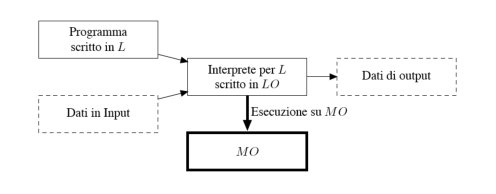
\includegraphics[scale=1.5]{interprete.pdf}
\end{center}

\noindent \textbf{Definizione:} dato $P^L \in Prog^L$ e $input \in D$, un interprete $int^{Lo, L}$ per $L$ in $Lo$ è un programma tale che $int ^{Lo, L} : (Prog^L x D) \rightarrow D$ e $int ^{Lo, L}(P^L, input) = P^L(input)$.\\

\noindent Le operazioni svolte dall'interprete sono:
\begin{itemize}
\item[-] Elaborazione dei dati primitivi, ovvero dei dati rappresentabili in modo diretto nella memoria tramite le operazioni aritmetiche (primitive) fornite dalla macchina stessa;
\item[-] Controllo di sequenza delle esecuzioni, effettuato tramite strutture dati (come quelle per la memorizzazione dell'indirizzo della prossima istruzione) manipolate con operazioni specifiche (come l'aggiornamento dell'indirizzo);
\item[-] Controllo dei dati, che consiste nel recupero dei dati necessari all'esecuzione delle istruzioni;
\item[-] Controllo della memoria.
\end{itemize}

\newpage

Il seguente pseudocodice descrive come opera generelmente un interprete:
\lstset{language=Java}
\begin{lstlisting}
begin    
  go := true; 
  while go do begin
	FETCH(OPCODE,OPINFO) at PC 	
	DECODE(OPCODE,OPINFO) 
	if OPCODE needs ARGS then FETCH(ARGS) 
	case OPCODE of 
		OP1: EXECUTE(OP1,ARGS) 
		... 
		OPn: EXECUTE(OPn,ARGS) 
		HLT: go:= false; 
	if OPCODE hasresultthen STORE(RES); 
	PC := PC + SIZE(OPCODE);     
  end(while)
end(begin)
\end{lstlisting}

Le operazioni svolte all'interno del ciclo \textbf{while} sono quindi: 
\begin{enumerate}
\item Acquisizione della prossima istruzione da eseguire;
\item Decodifica dell'istruzione per estrarre l'operazione e gli operandi;
\item Recupero degli operandi;
\item Esecuzione dell'operazione;
\item Memorizzazione dell'eventuale risultato in memoria;
\item Ripetizione dei punti sopra fino ad una operazione di "halt".
\end{enumerate}

\begin{center}
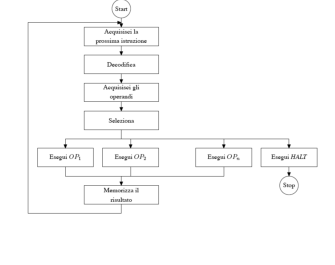
\includegraphics[scale=2.2]{interprete_struttura.pdf}
\end{center}

\noindent Caratteristiche: nessun costo di
traduzione, esecuzione lenta, scarsa efficienza della
macchina $M_L$, buona flessibilità e portabilità, facilità nell'interazione a run-time (es. debugging).

\item[-] \textbf{Soluzione compilativa}: si basa sull'utilizzo di un compilatore, definito come un programma $comp^{Lo, L}$ che traduce, preservando la semantica, programmi scritti nel linguaggio $L$ in programmi scritti nel linguaggio $Lo$, e quindi eseguibili direttamente sulla macchina astratta per $Lo$.

In questo caso la traduzione è esplicita, in quanto il codice in $Lo$ viene prodotto in output (e non eseguito).

\begin{center}
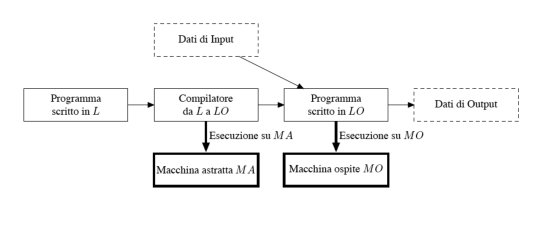
\includegraphics[scale=1.5]{compilatore.pdf}
\end{center}

\noindent \textbf{Definizione:} dato $P^L \in Prog^L$, un compilatore $comp^{Lo, L}$ da $L$ a $Lo$ è un programma tale che $comp^{Lo, L}: Prog^L \rightarrow Prog^{Lo}$ e $comp^{Lo, L}(P^L) = P^{Lo}$ tale che $\forall input \in D$ allora $P^{Lo}(input) = P^L(input)$.\\

Le fasi eseguite da un compilatore sono: 
\begin{itemize}
\item[-] Analisi lessicale (\textbf{Scanner}): spezza  un  programma  nei componenti   sintattici   primitivi  chiamati tokens (identificatori,   numeri, parole riservate, ...);
\item[-] Analisi sintattica (\textbf{Parser}): crea una rappresentazione ad albero  della  sintassi  del  programma  dove  ogni  foglia  è un  token  e  le  foglie  lette  da  sx  a  dx  costituiscono  frasi ben  formate  del  linguaggio. L'albero creato costituisce  la struttura logica del programma. Quando non è possibile costruire l’albero significa che qualche frase è illegale e la compilazione si blocca con un errore.
\end{itemize}

\begin{center}
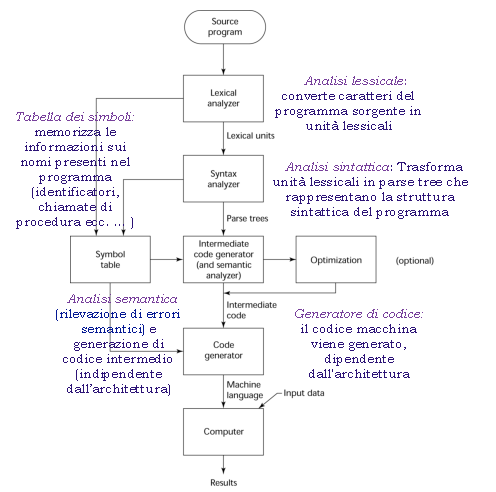
\includegraphics[scale=1.5]{compilatore_struttura.pdf}
\end{center}

\noindent Caratteristiche: costi di traduzione, esecuzione veloce, progettazione difficile, dipendente
dalla distanza fra $L$ e $Lo$, buona efficienza (decodifica a
carico del compilatore e ottimizzazioni), scarsa
flessibilità, perdita di informazione sulla struttura del
programma sorgente.

\newpage

\item[-] \textbf{Soluzione ibrida}: si basa sulla compilazione del linguaggio ad alto livello in un linguaggio intermedio (di più basso livello), che viene poi interpretato.

\begin{center}
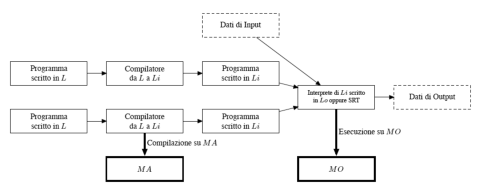
\includegraphics[scale=1.5]{ibrido.pdf}
\end{center}

\end{itemize}

\subsubsection*{Specializzatore}
Lo specializzatore valuta un programma su una parte dell'input, ottenendo un programma più efficiente su quella parte dell'input. Lo specializzatore effettua quindi delle trasformazioni all'interno dello stesso linguaggio (Valutazione parziale).

É stato dimostrato che è possibile caratterizare un compilatore a partire da un interprete e uno specializzatore: specializzando un interprete rispetto al programma si ottiene un compilatore.







\end{document}